\documentclass[mathserif]{beamer}
\usetheme[secheader]{pecostalk}

\newcommand{\commentout}[1]{}

\usepackage{amsmath}
\usepackage{color}
% \usepackage{minted} % On Mac: error, you must have pygmentize installed to use this package

\usepackage{xspace}
\newcommand{\libMesh}{\texttt{libMesh}\xspace}
\newcommand{\orderof}[1]{\ensuremath{ {\cal O}\left(#1\right)}}

\newcommand{\abs}[1]{\ensuremath{ \left|#1\right|}}
\newcommand{\norm}[1]{\ensuremath{ \left|\left|#1\right|\right|}}
\newcommand{\bv}[1]{{\boldsymbol{#1}}}
\newcommand{\Reals}{\mathbb{R}}

\newcommand{\Qoi}{{\ensuremath{Q}}}
\newcommand{\qoi}{{\ensuremath{q}}}
\newcommand{\Res}{{\ensuremath{\mathcal R}}}
\newcommand{\params}{{\ensuremath{\bv{\xi}}}}
\newcommand{\Unknowns}{{\ensuremath{\bf{U}}}}
\newcommand{\unknown}{{\ensuremath{\bv{u}}}}
\newcommand{\Testfuncs}{{\ensuremath{\bf{V}}}}
\newcommand{\primalsol}{{\ensuremath{\bv{\tilde{u}}}}}
\newcommand{\primalsolh}{{\ensuremath{\bv{\tilde{u}^h}}}}
\newcommand{\adjointsol}{{\ensuremath{\bv{\tilde{z}}}}}
\newcommand{\adjointsolh}{{\ensuremath{\bv{\tilde{z}^h}}}}
\newcommand{\adjointsolH}{{\ensuremath{\bv{\tilde{z}^H}}}}
\newcommand{\Liftfunc}{{\ensuremath{\Psi}}}
\newcommand{\elem}{\ensuremath{E}}

\definecolor{DarkGreen}{rgb}{0.13,0.55,0.13}
\definecolor{DarkRed}{rgb}{0.55,0.13,0.13}
\newcommand{\pro}[1]{{\color{DarkGreen}{#1}}}
\newcommand{\con}[1]{{\color{DarkRed}{#1}}}

\graphicspath{{./figs/}}

\date{Feb 26, 2016}
\author{Roy H.~Stogner\inst{1}}
\institute{\inst{1}The University of Texas at Austin}
\title[libMesh]{PDE Discretization and Analysis with libMesh}
\begin{document}

\begin{frame}
\begin{center}

\includegraphics[width=.8\linewidth]{grand_logo}\\
\end{center}
\titlepage
\end{frame}

%\AtBeginSection[]
%{
%   \begin{frame}
%       \frametitle{Outline}
%       \tableofcontents[currentsection]
%   \end{frame}
%}

%===============================================================================
\section{Introduction}
%===============================================================================


\begin{frame}{libMesh Finite Element Library}
\begin{columns}
\column{.4\textwidth}
\begin{block}{Scope}
\begin{itemize}
\item Free, Open source
\begin{itemize}
\item LGPL2 for core
\end{itemize}
\item 35 Ph.D.\ theses, 393 papers (58 in 2015)
\item $\sim10$ current developers
\item $160-240$ current users?
\end{itemize}
\end{block}

\column{.6\textwidth}
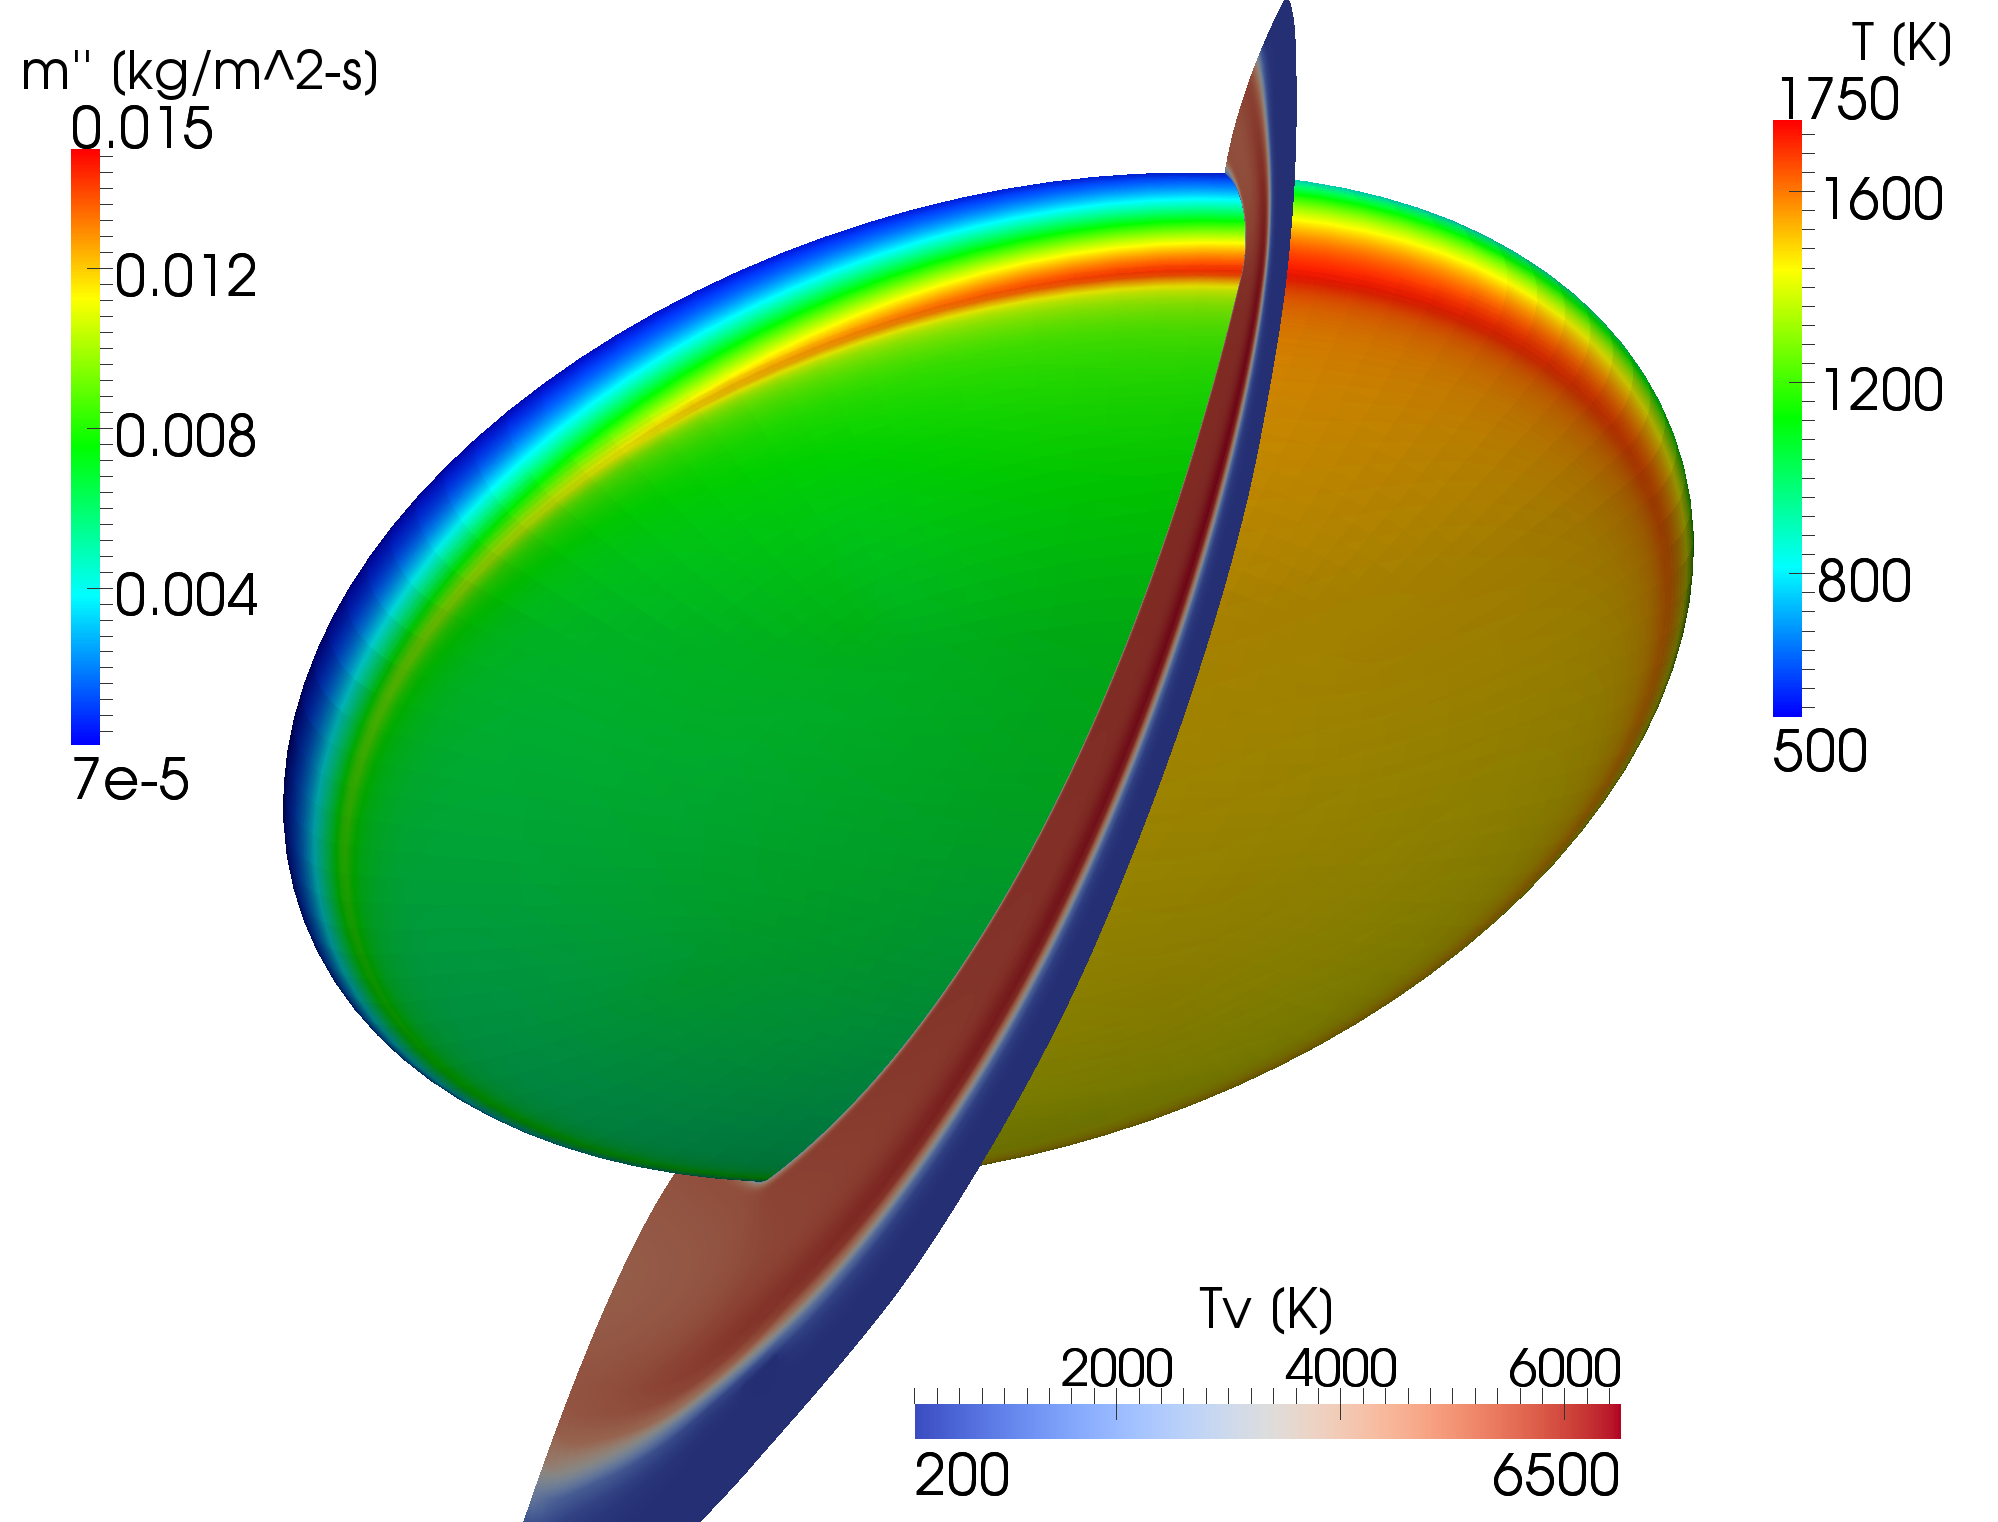
\includegraphics[width=.45\textwidth]{ablating_hs_wbg}
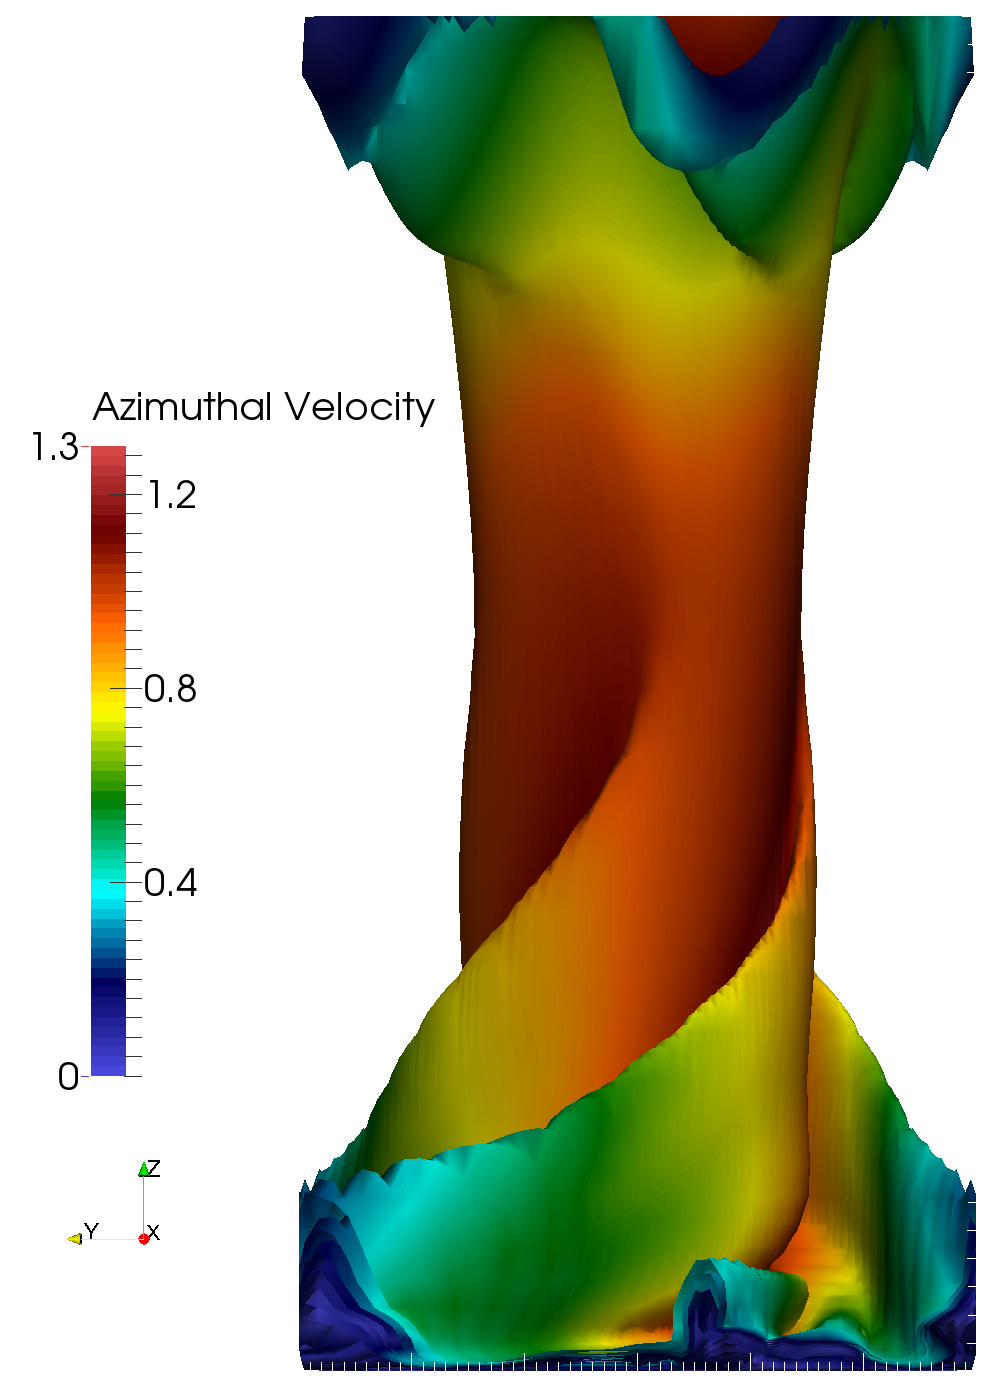
\includegraphics[width=.25\textwidth]{sov}
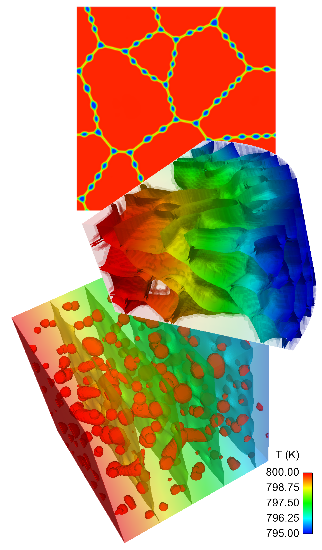
\includegraphics[width=.3\textwidth]{marmot1b}
\end{columns}

\begin{columns}
\column{.35\textwidth}
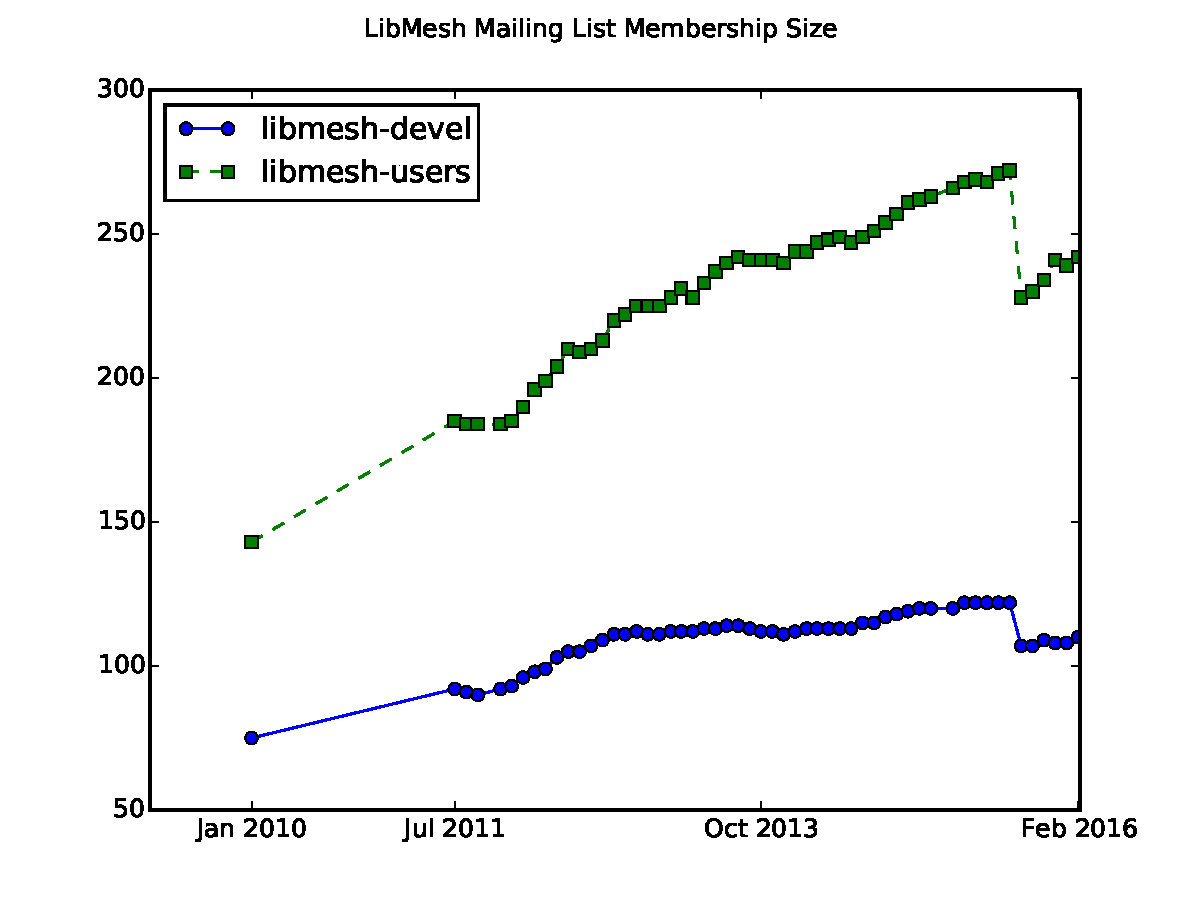
\includegraphics[width=\textwidth]{libmesh_mailinglists_membership}

\column{.65\textwidth}
\begin{block}{Challenges}
\begin{itemize}
\item Radically different application types
\item Widely dispersed core developers
\begin{itemize}
\item INL, UT-Austin, U.Buffalo, JSC, MIT, Harvard, Argonne
\end{itemize}
\item OSS, commercial, private applications
\end{itemize}
\end{block}
\end{columns}

\end{frame}

\begin{frame}[t]
  \begin{columns}
    \column{.6\textwidth}
    \begin{center}
      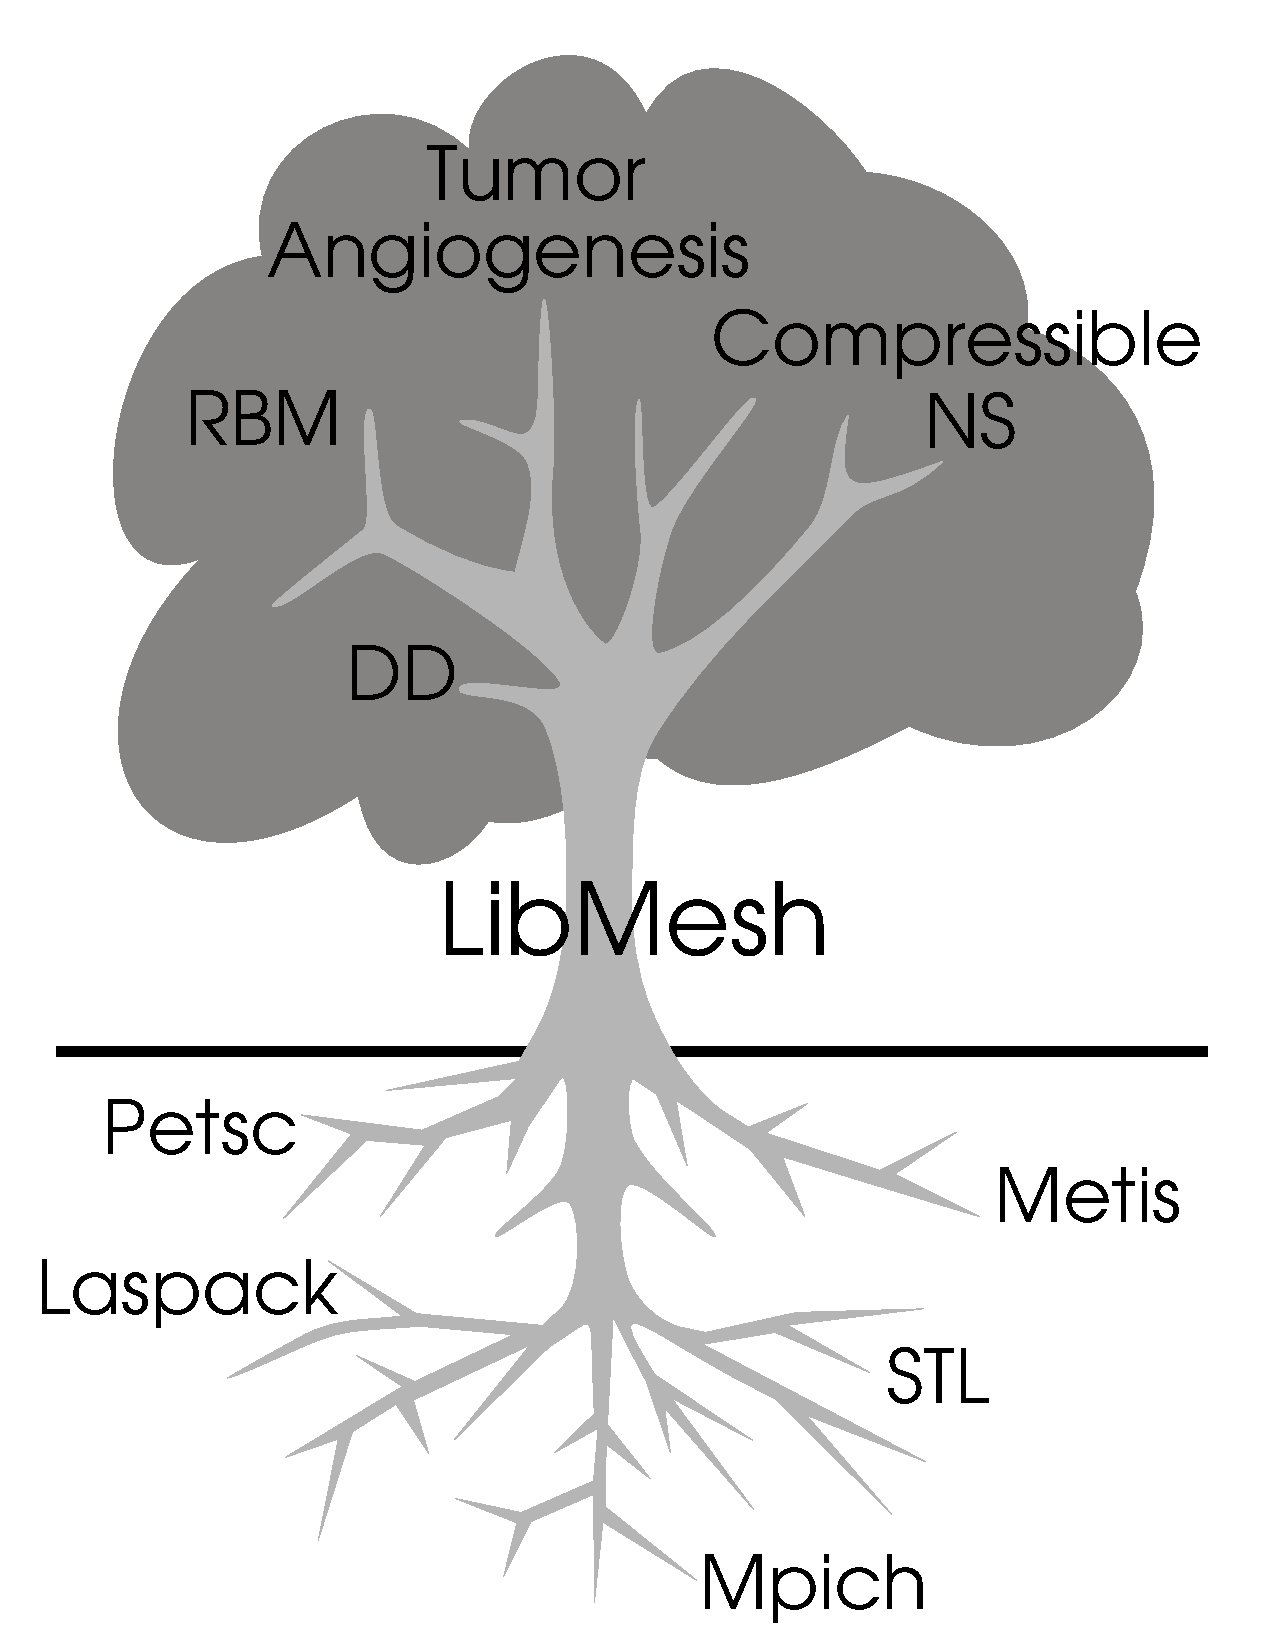
\includegraphics[width=.9\textwidth]{mytreeandroots_allnames}
    \end{center}
    \column{.35\textwidth}
    \begin{itemize}
      \item Foundational (typically optional) library access via LibMesh's ``roots''.
      \item Application ``branches'' built off the library ``trunk''.
      \item Additional middleware layers (e.g. Akselos, GRINS, MOOSE) for more complex applications
    \end{itemize}
  \end{columns}

\end{frame}



\begin{frame}[t]
  \frametitle{Typical Boundary Value Problem}
  \begin{columns}[t]
    \column{.5\textwidth}
     \begin{itemize}
      \item Common BVP components:
      \vspace{-.1in}
        \begin{eqnarray}
	\label{eqn:general_pde}
	\nonumber
	\bv{M} \frac{\partial \bv{u}}{\partial t} & = & \bv{F}( \bv{u} ) \;\, \in \Omega \subset \Reals^n
        \\
	\nonumber
	\bv{G}( \bv{u} ) & = & 0 \;\;\;\;\;\;\;\; \in \Omega
	\\
	\nonumber
	\bv{u} & = & \bv{u}_D \;\;\;\;\; \in \partial \Omega_D
	\\
	\nonumber
	\bv{N}(\bv{u}) & = & 0 \;\;\;\;\;\;\;\; \in \partial \Omega_N
 	\\
 	\nonumber
 	\bv{u}(\bv{x}, 0) & = & u_0(\bv{x}) 
      \end{eqnarray}
      \item Less common components:
        \begin{itemize}
        \item Moving domain $\Omega(t)$, $\Omega(\bv{u},t)$
        \item Multi-dimensional manifolds
        \item Self-overlapping, contact
        \item Acceleration ${\partial^2 u}/{\partial t^2}$
        \item Integro-differential equations
        \end{itemize}
      \end{itemize}
%    \end{block}
    %\pause
    \column{.5\textwidth}
      \begin{center}
	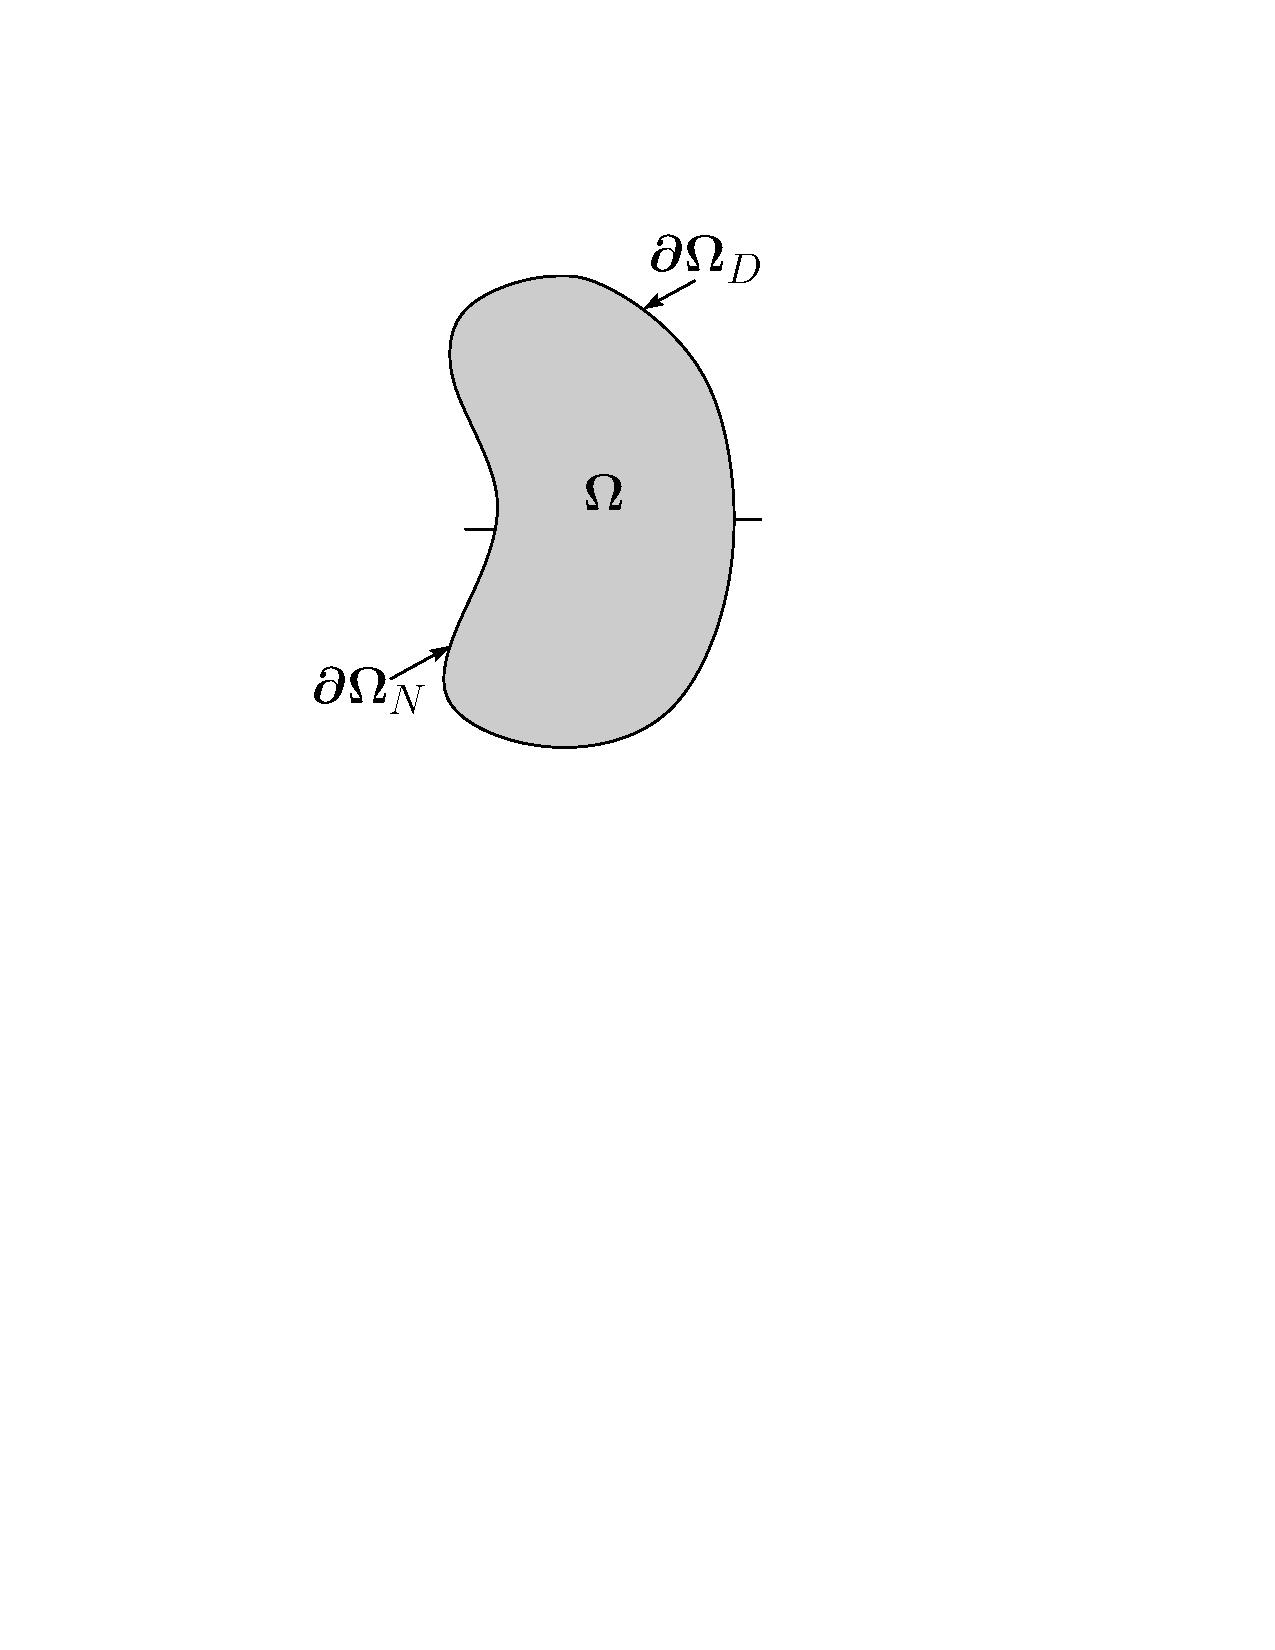
\includegraphics[viewport=140 420 400 685,clip=true,width=.5\textwidth]{domain2_input}
	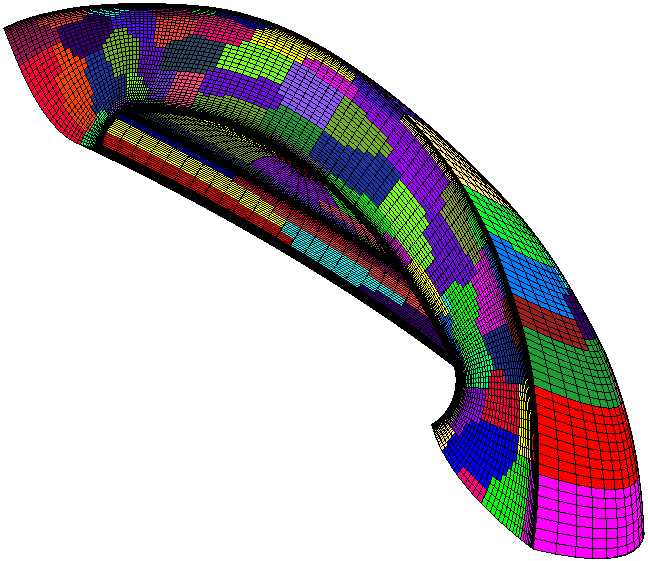
\includegraphics[width=.5\textwidth]{capsule_partitioned}

	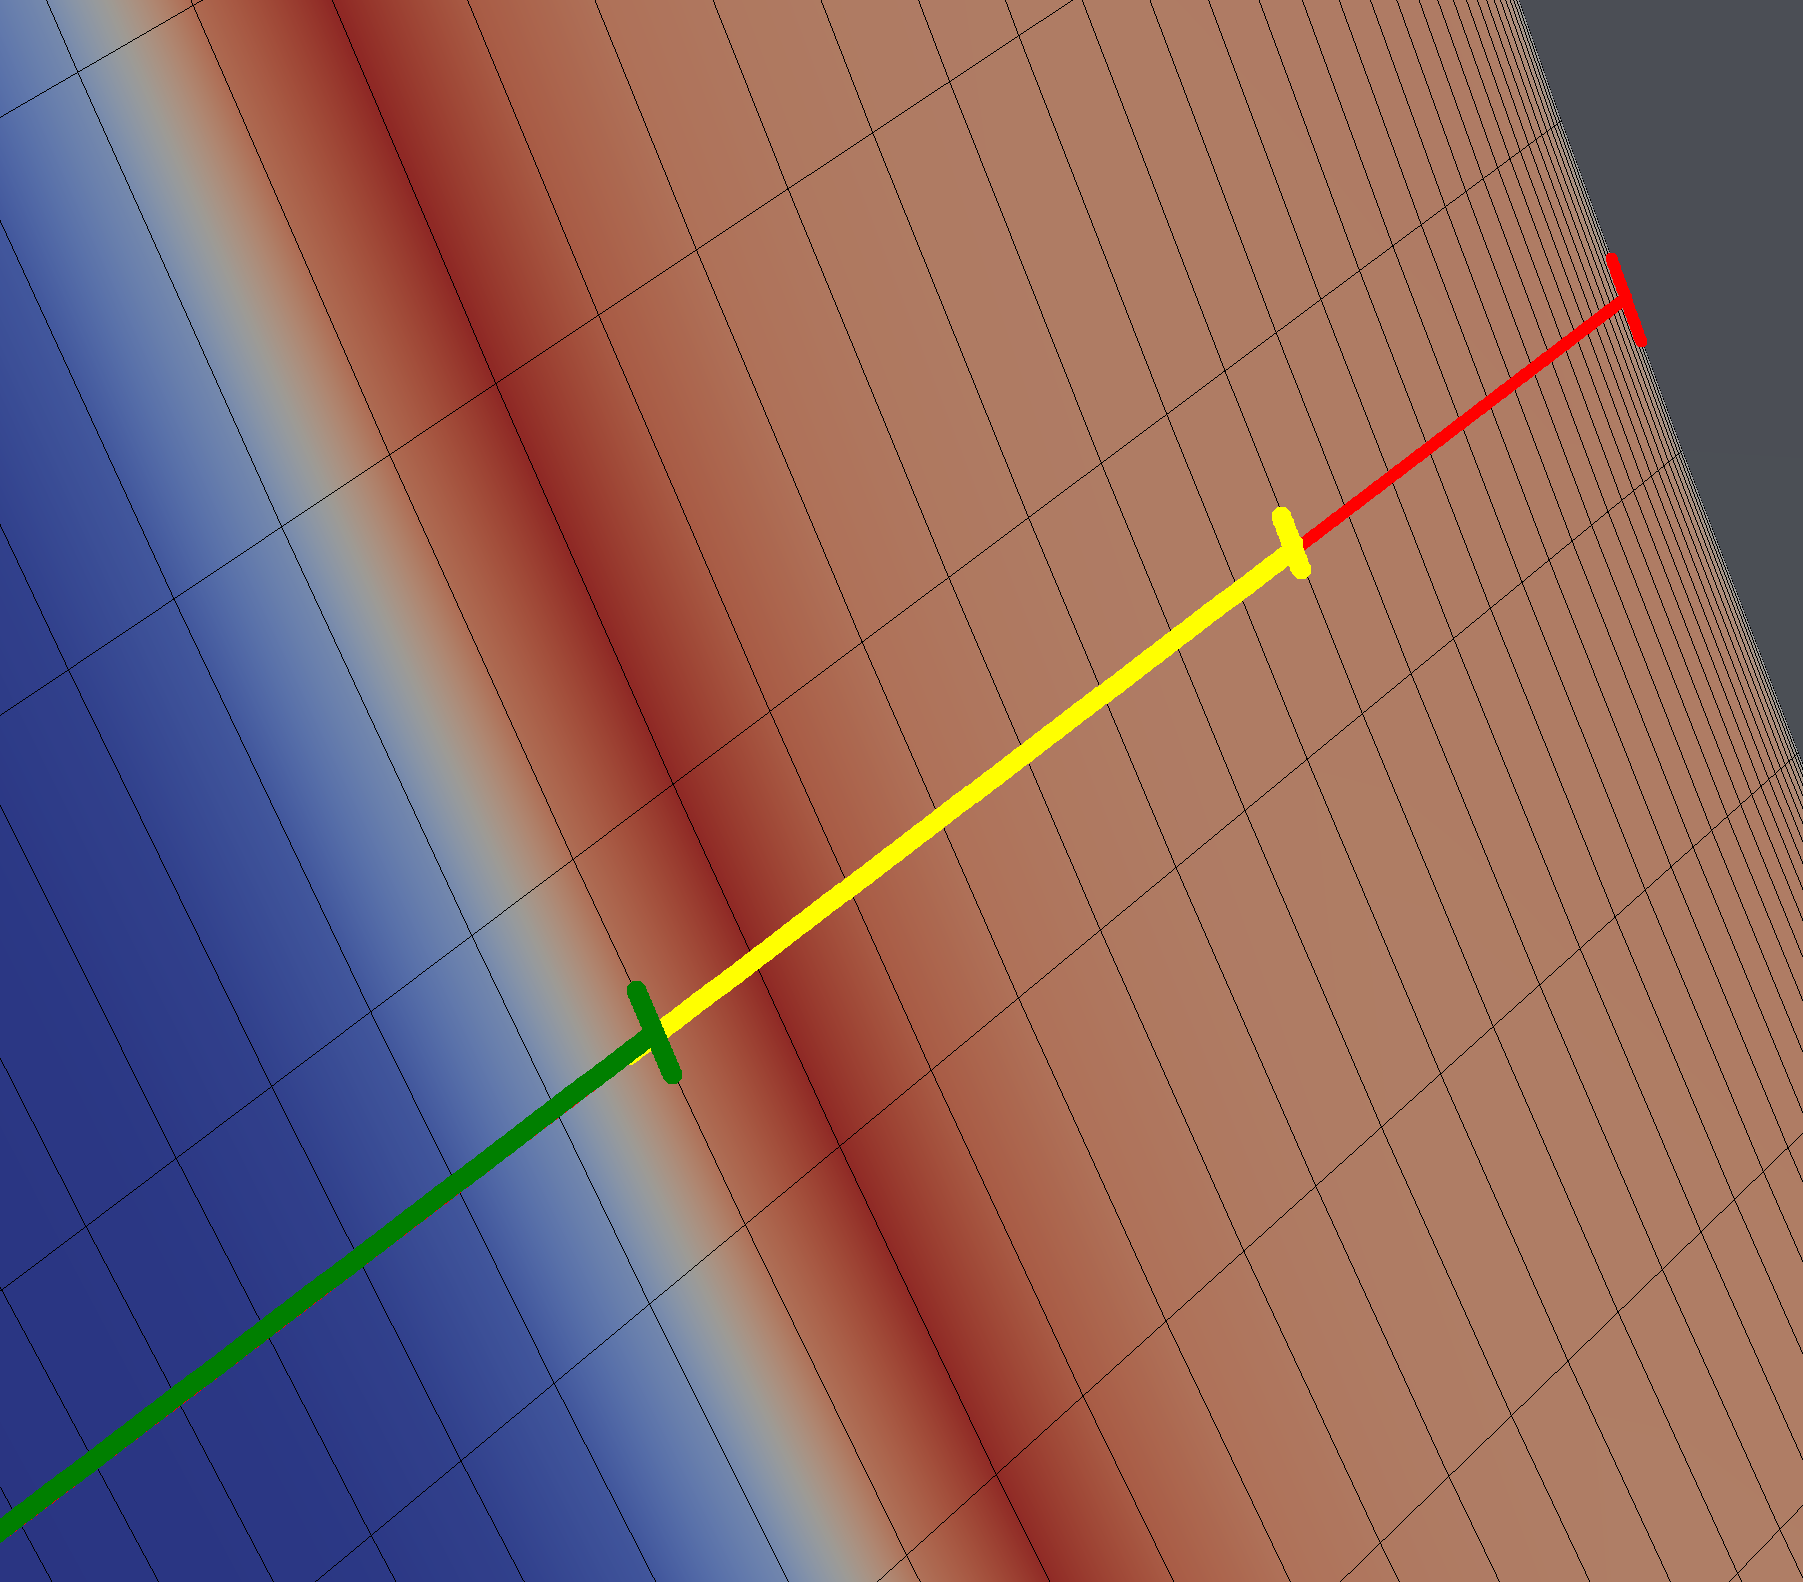
\includegraphics[width=.45\textwidth]{fins-transition} \;
	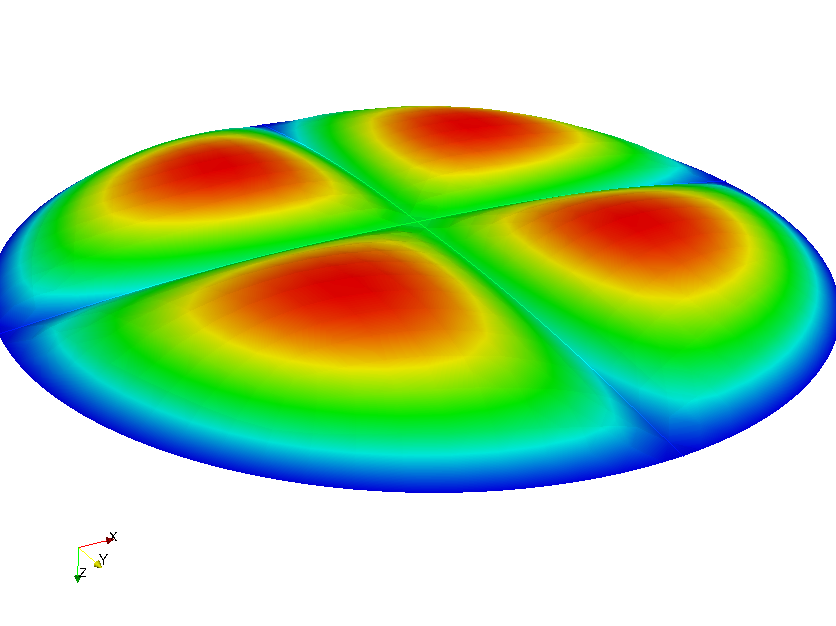
\includegraphics[width=.45\textwidth]{sheet_perspective}

      \end{center}
  \end{columns}
\end{frame}


\begin{frame}
\frametitle{Mesh Classes}
\begin{columns}
\column{.6\textwidth}
\begin{center}
\includegraphics[width=.95\textwidth]{MeshUML}
\end{center}
\column{.4\textwidth}
%\begin{block}{}
\begin{itemize}
\item \texttt{MeshBase} gives node or element iterators, all or active, global or local
\item \texttt{SerialMesh} or \texttt{ParallelMesh} manages synchronized or distributed data
\end{itemize}

\includegraphics[width=.75\textwidth]{ParallelMesh3}
%\end{block}
\end{columns}

\end{frame}


\begin{frame}
\frametitle{Geometric Element Classes}

\begin{columns}
\column{.55\textwidth}
\begin{center}
\vspace{-5mm}
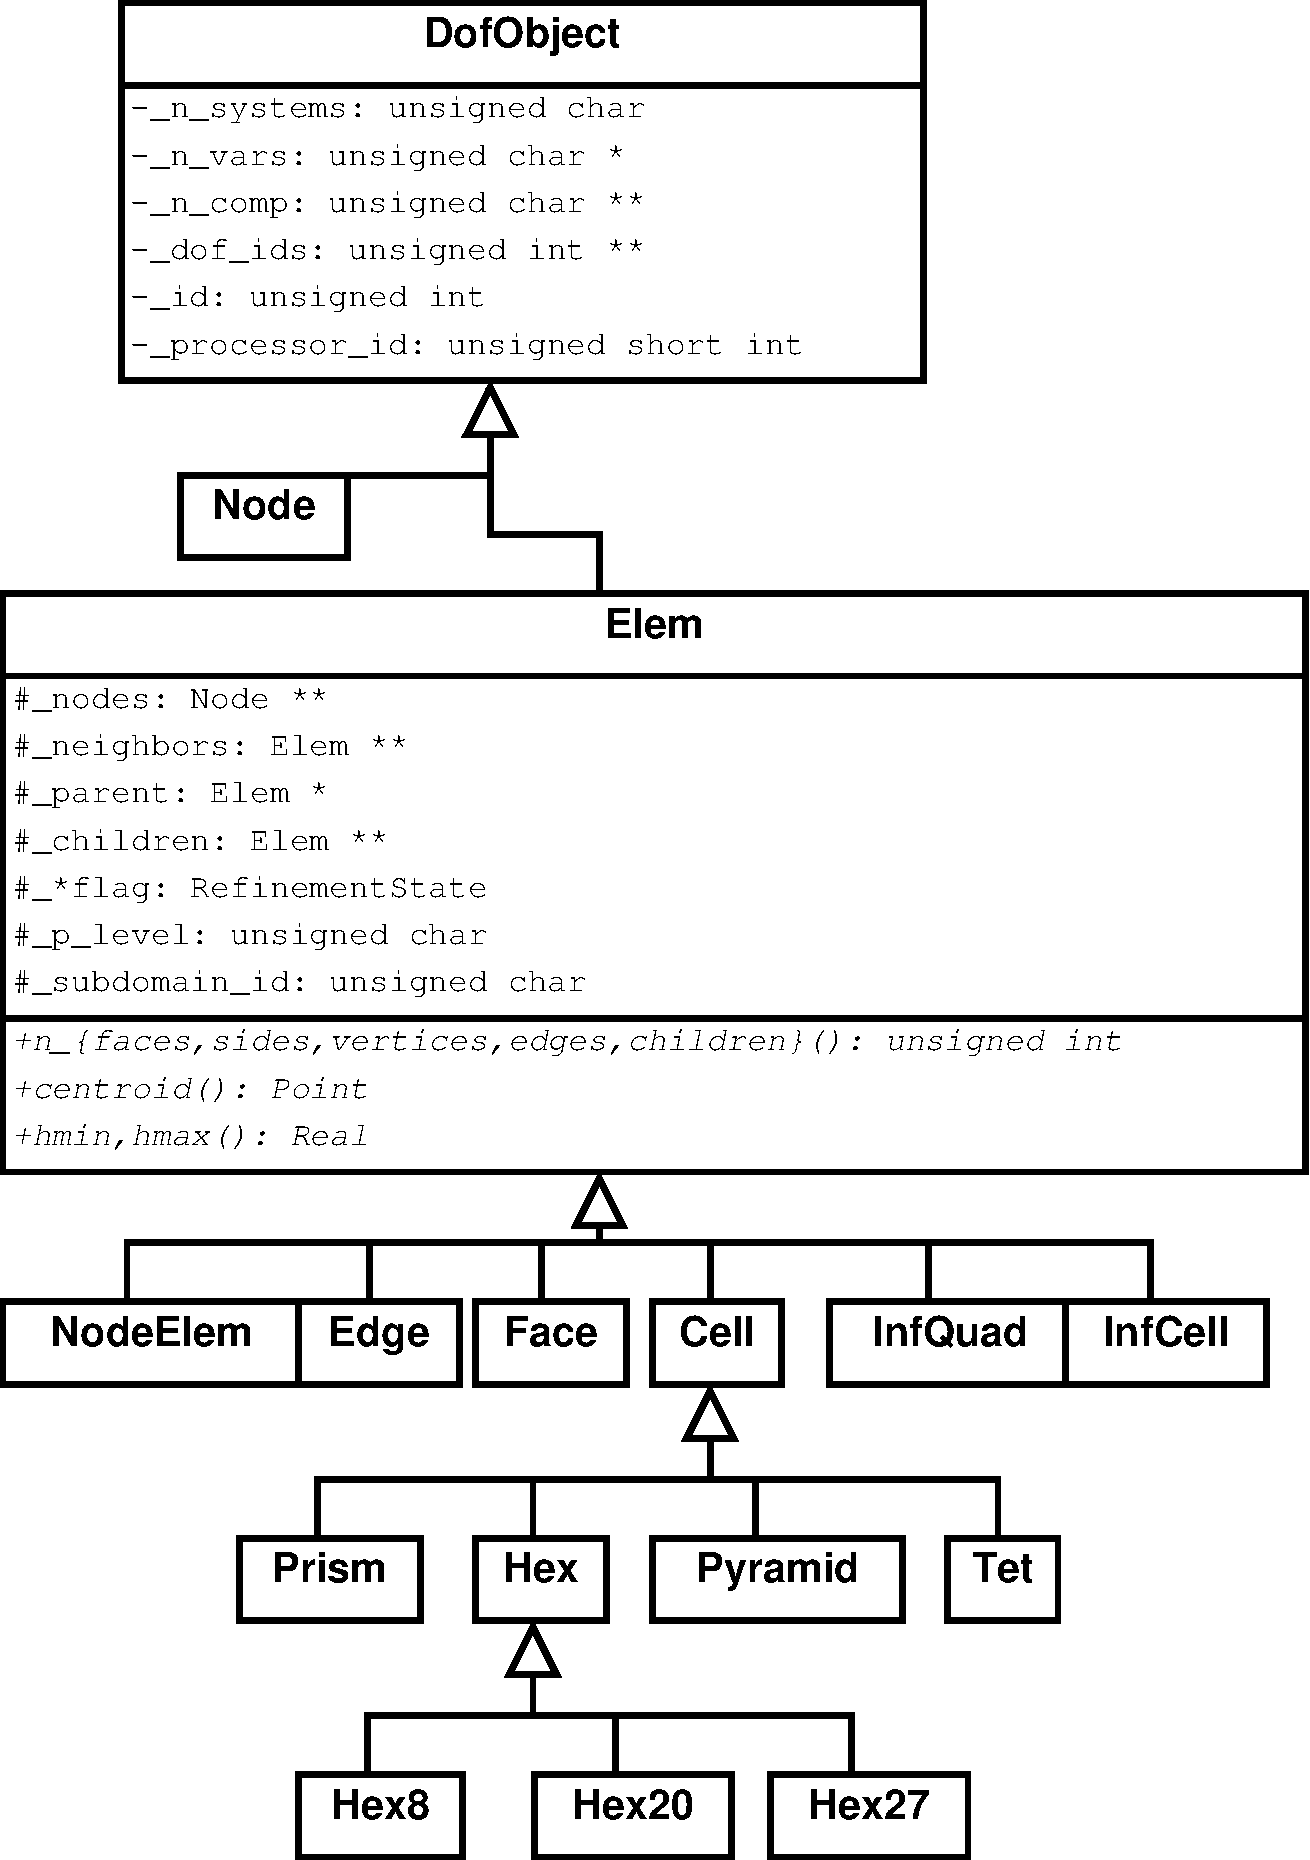
\includegraphics[width=.75\textwidth]{DofObjects}
\end{center}
\column{.45\textwidth}
\begin{itemize}
\item Abstract interface gives mesh topology
\item Concrete instantiations of mesh geometry
\item Hides element type from most applications
\item Base class data arrays allow more optimization, inlining
\end{itemize}

Similar trees:

\begin{itemize}
\item Shape functions, quadrature
\item Periodic boundary maps
\item Reference counts, comms
\item Linear algebra, solvers
\item Integrators, strategies
\end{itemize}
\end{columns}

\end{frame}


\begin{frame}%[<+->]
  \frametitle{Poisson Example}
  \begin{itemize}
  \item {Consider the weak form arising from the Poisson equation,
    \begin{eqnarray}
      \nonumber
      \Res( u, v ) := \hspace{2.5in} \\  \nonumber
      \int_{\Omega^h}  \left[ \nabla u \cdot \nabla v - f v \right] dx %\\ \nonumber
      %+ \int_{\partial \Omega^h_N} u_N v^h \;ds
      =0 \hspace{.5in} \forall v \in \mathcal{V}
    \end{eqnarray}
  }
  \end{itemize}
\end{frame}


\begin{frame}[fragile,t]  
  \frametitle{Poisson Example}
%	\begin{block}{}
	  \begin{itemize}    
	  \item{ The LibMesh representation of the matrix and
	    rhs assembly is similar to the mathematical statements.
	  }
	  \end{itemize}
%	\end{block}
\small
\begin{semiverbatim}
for (q=0; q<Nq; ++q) 
  for (i=0; i<Ns; ++i) \{
    \alert<2>{Fe(i)   += JxW[q]*f(xyz[q])*phi[i][q];}
    
    for (j=0; j<Ns; ++j)
      \alert<3>{Ke(i,j) += JxW[q]*(dphi[j][q]*dphi[i][q]);}
  \}
\end{semiverbatim}
\only<2>
{
  \begin{equation}
    \nonumber
    \bv{F}^e_{i} = 
    \sum_{q=1}^{N_q}
    f(x(\xi_q))
    \phi_i(\xi_q)
    |J(\xi_q)| w_q
  \end{equation}
}
\only<3->
{
  \begin{equation}
  \nonumber
  \bv{K}^e_{ij} =
  \sum_{q=1}^{N_q}
    \nabla \phi_j(\xi_q) \cdot
    \nabla \phi_i(\xi_q)
    |J(\xi_q)| w_q
  \end{equation}
}
\end{frame}


%===============================================================================
\begin{frame}
\frametitle{Scalability: Hybrid MPI + Threads}

\begin{columns}
\column{.65\textwidth}
\begin{block}{Parallel:: interfaces wrap MPI}
Library data is distributed, synchronized:
\begin{itemize}
	\item Simpler, STL-compatible, inlined API
	\item Works with complex serializable classes
\end{itemize}
\end{block}

\begin{block}{Threads:: interfaces TBB/pthreads/OpenMP}
\begin{itemize}
	\item Sparsity, AMR constraint calculation
	\item {\texttt{FEMSystem}} assembly routines
	\item Asynchronous I/O
	\item Mesh projections, utility functions
\end{itemize}
\end{block}

\column{.35\textwidth}
\center
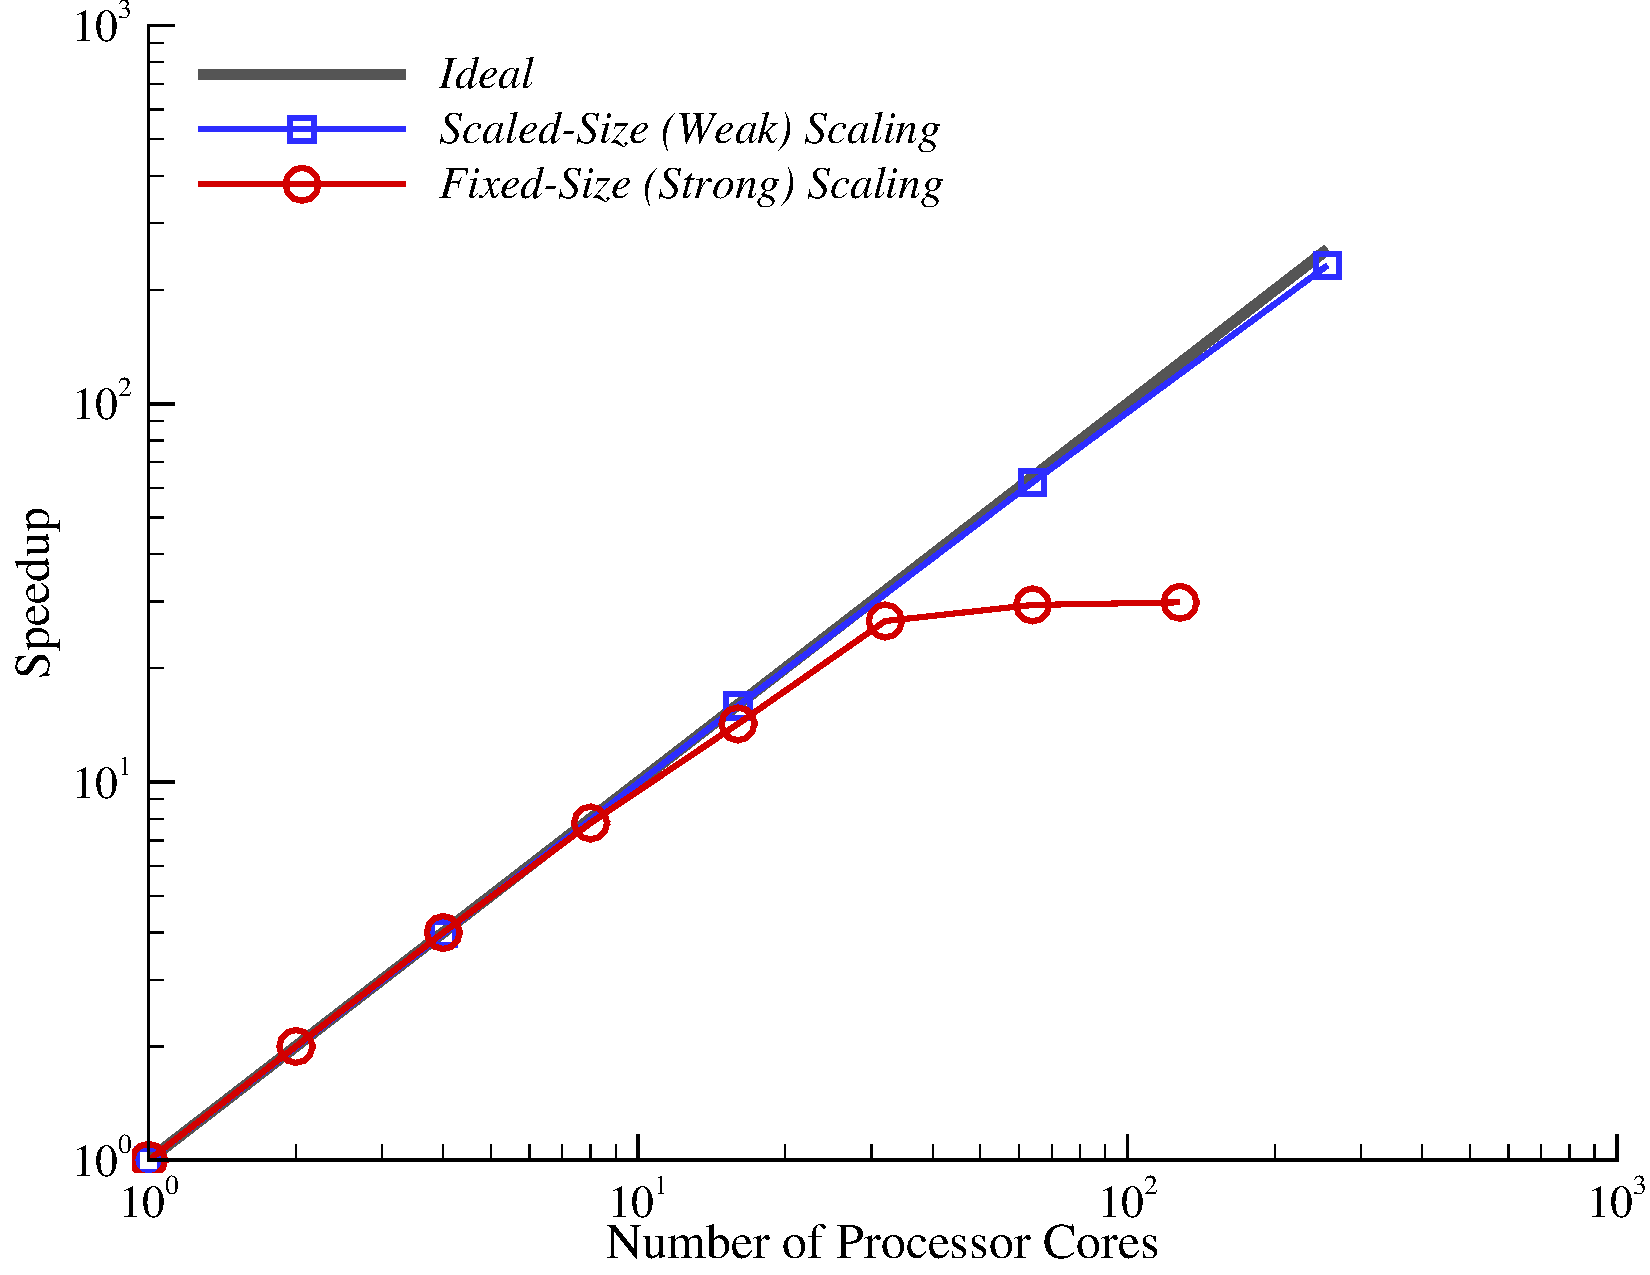
\includegraphics[width=.8\textwidth]{fins_speedup}

\center
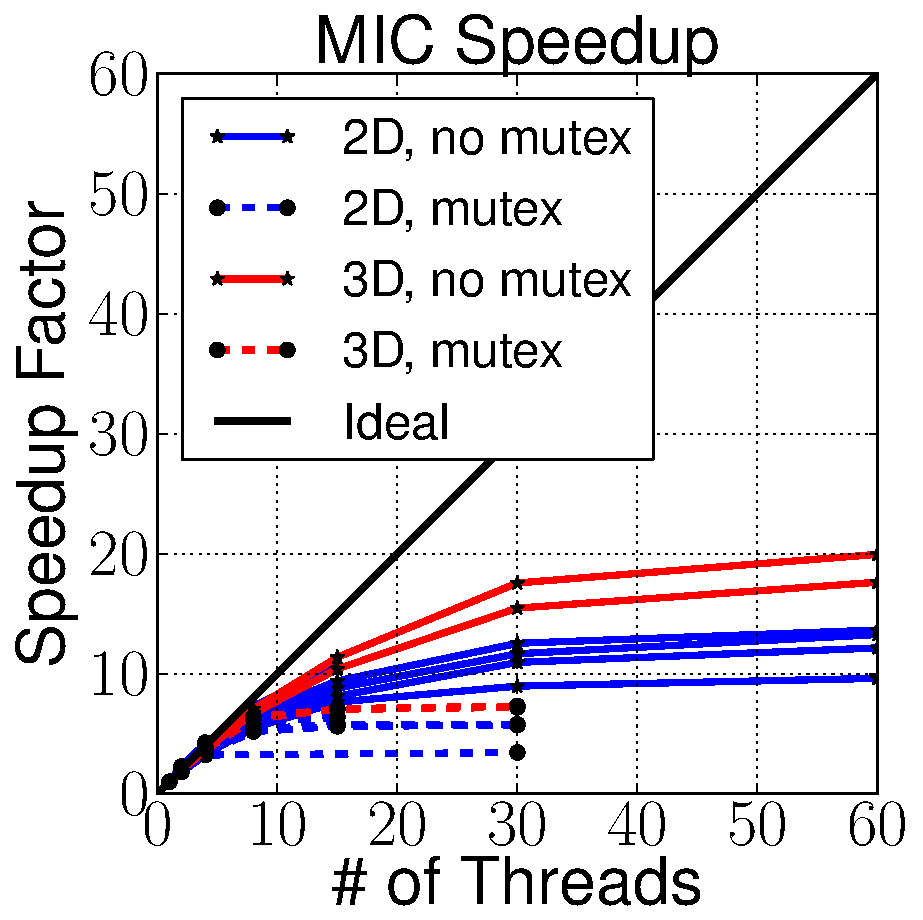
\includegraphics[width=.8\textwidth]{threaded_speedup}

\end{columns}

\begin{itemize}
	\item Hybrid parallel apps with {\emph{no}}
		threading or message passing code
	\item API-independence via \libMesh{} wrappers
\end{itemize}
\end{frame}




%===============================================================================
\section{Adaptivity}
%===============================================================================

\begin{frame}
\frametitle{Adaptivity: Error Estimators, Error Indicators}
\begin{columns}
\column{.7\textwidth}
\begin{block}{Error decompositions}
	Subterms on each element $K$:
	\begin{itemize}
		\item $\norm{u-u_h}_\mathcal{H}^2 = 
			\sum_K \norm{u-u_h}_\mathcal{H(K)}^2 \leq 
			\sum_K \abs{\eta_K}^2$
		\item $\Qoi(u) - \Qoi(u_h) \approx \sum_K \eta_K$
		\item $\abs{\Qoi(u) - \Qoi(u_h)} \leq \sum_K \abs{\eta_K}$
	\end{itemize}
\end{block}
\begin{block}{Refinement heuristics}
	\begin{itemize}
	\item Refinement/coarsening of elements with:
	\begin{itemize}
		\item Worst/best fraction sorted by error
		\item Error over/under fraction of tolerance
		\item Error over/under target mesh size average
	\end{itemize}
	\item $h$-vs-$p$ refinement:
	\begin{itemize}
		\item {\textit{a priori}} singularity identification
		\item Behavior vs. cost when $h$ vs. $p$ coarsening?
	\end{itemize}
	\end{itemize}
\end{block}

\column{.3\textwidth}
\center
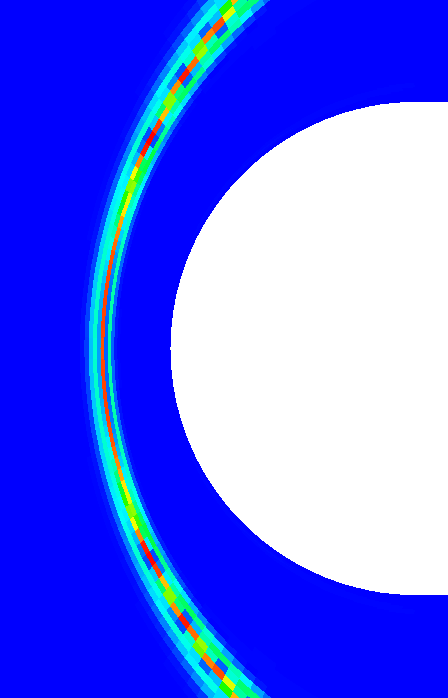
\includegraphics[width=.6\textwidth]{qoi_primal_error}

\center
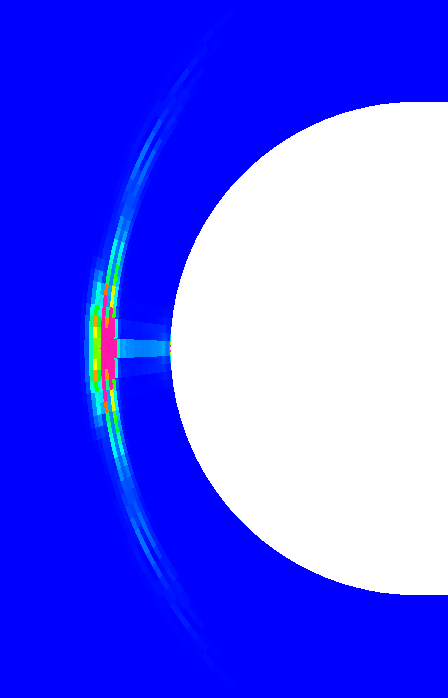
\includegraphics[width=.6\textwidth]{qoi_weighted_error}
\end{columns}
\end{frame}


\begin{frame}
\frametitle{Goal-oriented Adaptivity}

\begin{columns}

\column{0.5\textwidth}
Refine to reduce solution error {\emph{when it influences QoI error}}:

\begin{center}
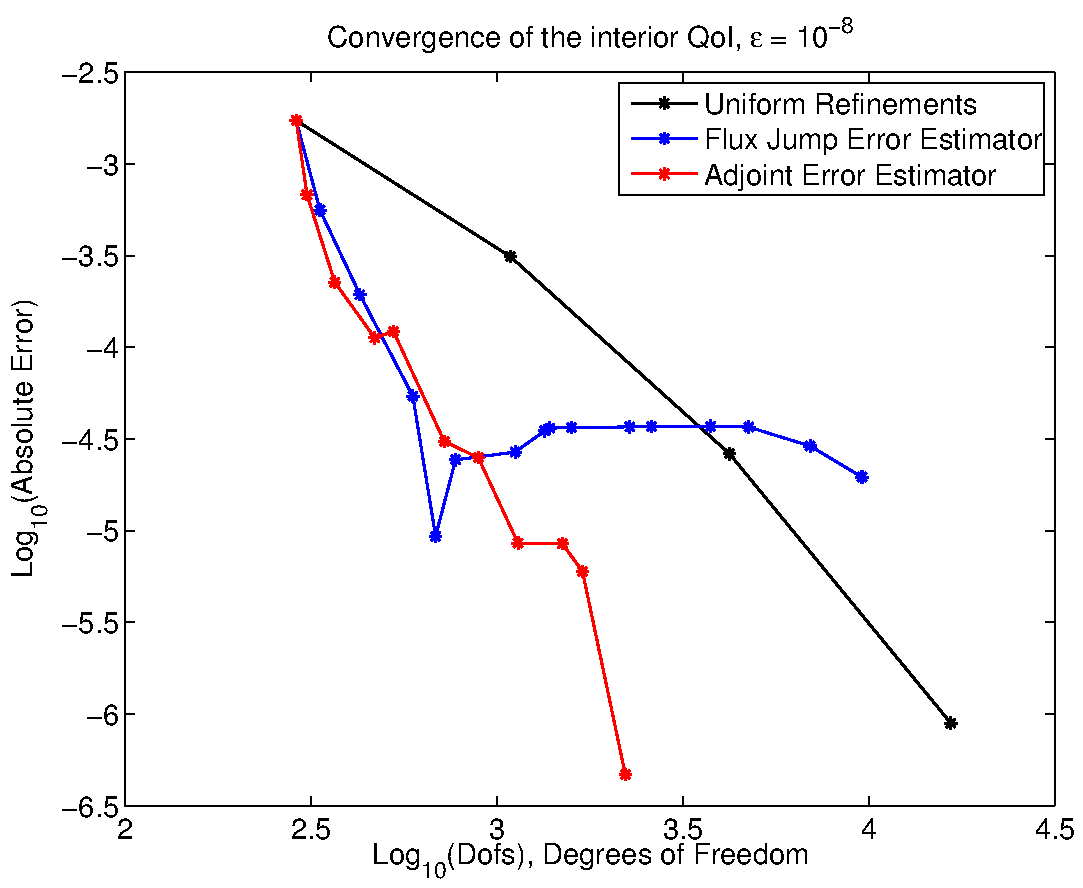
\includegraphics[width=1.0\textwidth]{qoi_may_29_2009_convergence_cropped}
\end{center}

\column{0.45\textwidth}

\begin{center}
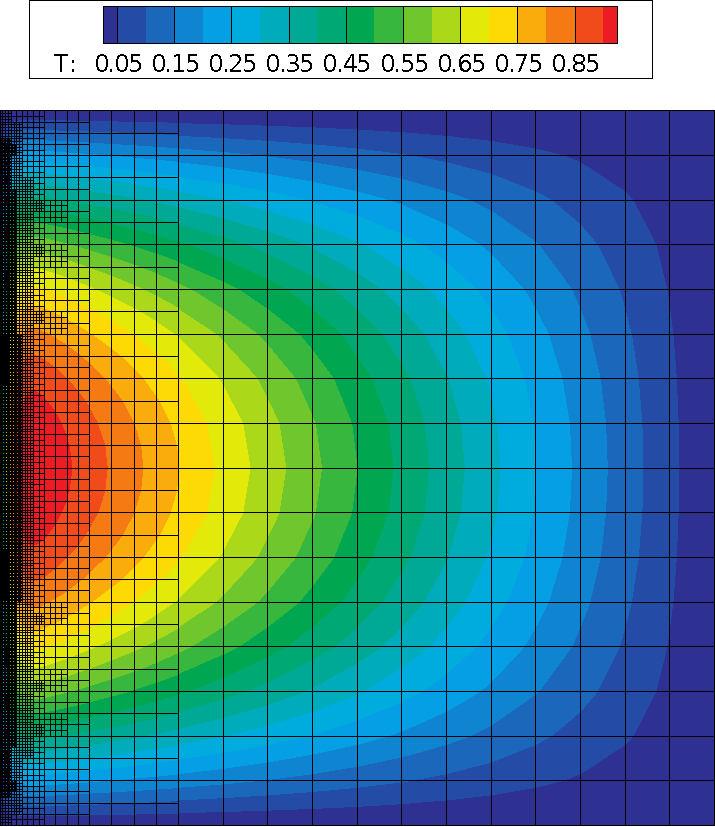
\includegraphics[height=0.5\textwidth]{QoI_October_20_2011_kelly_mesh}
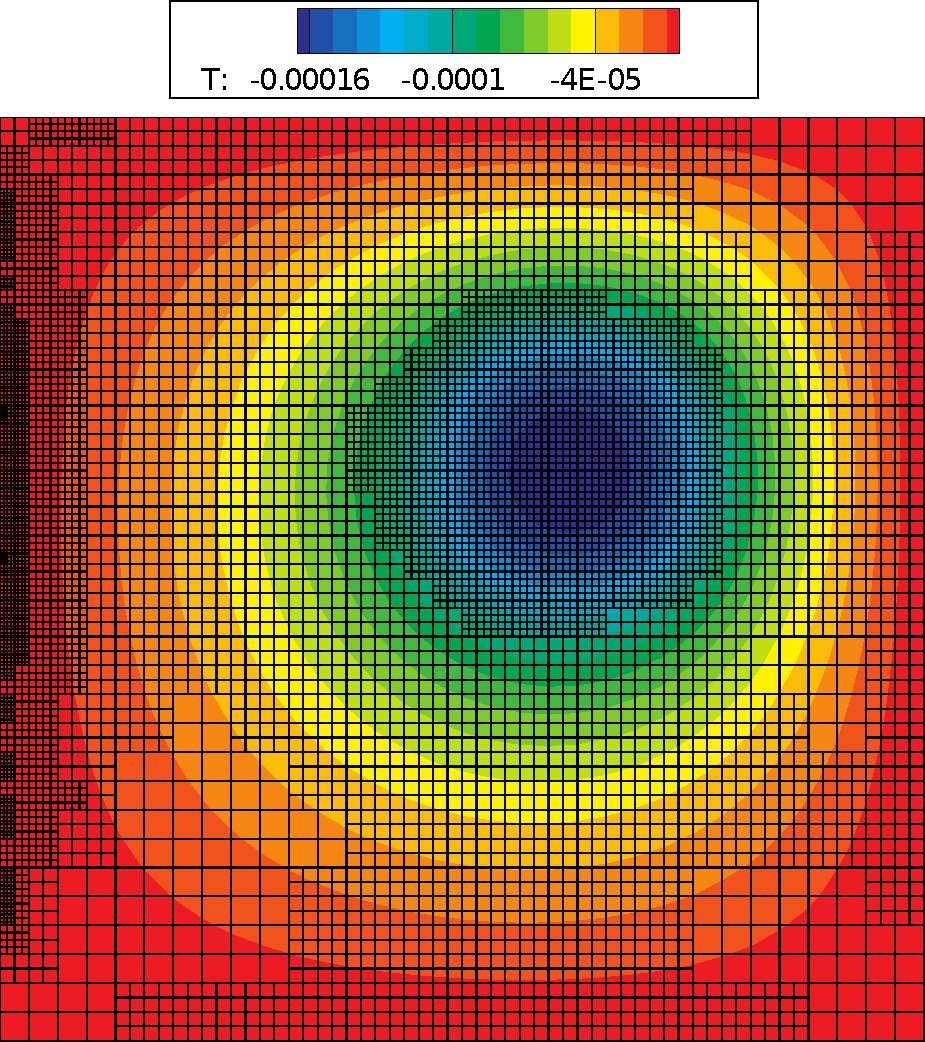
\includegraphics[height=0.5\textwidth]{QoI_May_29_2009_arpp_mesh+adjoint}
\end{center}

\begin{itemize}
\item Global error indicator targets layer alone; QoI temporarily plateaus
\item Rapid convergence from adjoint-based refinement
\end{itemize}

\end{columns}

\end{frame}


\begin{frame}
\frametitle{Adjoint-based Error Indicators, Sensitivities}

\vspace{-5mm}

\begin{eqnarray*}
\Qoi(\primalsolh) - \Qoi(\primalsol) & = & \Res(\primalsolh, \adjointsol - \adjointsolh) + H.O.T. \\
\qoi' & = & \Qoi_\params(\primalsol; \params) - 
        \Res_\params(\primalsol, \adjointsol - \Liftfunc(\primalsol; \params); \params)
\end{eqnarray*}

\begin{block}{Adjoint Refinement}
\begin{equation*}
\Res(\primalsolh, \adjointsol - \adjointsolh) \approx \sum_\elem 
\Res^\elem(\primalsolh, \adjointsolH - \adjointsolh)
\end{equation*}
\end{block}

\begin{block}{Adjoint Residual}
\vspace{-4mm}
\begin{equation*}
\abs{\Res(\primalsolh, \adjointsol - \adjointsolh)} \leq
\sum_\elem \norm{\Res^\elem_\unknown}_{B(\Unknowns^\elem,
\Testfuncs^{\elem *})}
\norm{\primalsol - \primalsolh}_{\Unknowns^\elem}
\norm{\adjointsol - \adjointsolh}_{\Testfuncs^\elem}
\end{equation*}
\end{block}

\begin{block}{Generalized Adjoint Residual}
\vspace{-4mm}
\begin{align*}
\abs{\Res(\primalsolh, \adjointsol - \adjointsolh)}
\leq \sum_\elem \norm{\adjointsol_i-\adjointsolh_i}_i \; M_{ij} \; \norm{\primalsol_j-\primalsolh_j
}_j \nonumber
\end{align*}
\end{block}

\end{frame}



%===============================================================================
\section{Collaboration Strategies}
%===============================================================================


%===============================================================================
% NEW SLIDE
%===============================================================================
\begin{frame}
\frametitle{Collaboration Strategies}

\begin{block}{Communication}
\begin{itemize}
	\item Face to face, instant messaging, teleconference
	\item Email lists
	\begin{itemize}
		\item \texttt{libmesh-users@sourceforge.net},
			\texttt{libmesh-devel@sourceforge.net}
	\end{itemize}
	\item Trac/Redmine/Sourceforge issue tracking
	\item GitHub issues
\end{itemize}
\end{block}

\begin{block}{Code}
\begin{itemize}
	\item Email attachments
	\item Ticket attachments
		\item Repository forks!
		\item Pull requests!
\end{itemize}
\end{block}

\end{frame}



%===============================================================================
\section{Source Code Control}
%===============================================================================

%\begin{frame}{}
%  \begin{itemize}\itemsep=.05\textheight
%  \item When discussing SCC software, the distinction between ``distributed'' and ``centralized''
%    is often stressed, perhaps unnecessarily. 
%  \item Distributed SCC software, like \texttt{git}, is very frequently used in a semi-centralized manner.
%  \item The \libMesh library is now distributed from GitHub\footnote{\url{https://github.com/libMesh/libmesh}},
%    and therefore we focus on \texttt{git} in this talk, but the discussion should apply to other
%    SCC software as well.
%  \end{itemize}
%\end{frame}


%\subsection{Attention Deficit Development}
%\begin{frame}
%  \begin{itemize}\itemsep=.05\textheight
%  \item A more intrinsic difference between various flavors of SCC software is rather the ability to
%    make ``local commits.''
%  \item \texttt{git} and other ``distributed'' SCC software packages (\texttt{hg}) have this feature.
%  \item SVN lacks this feature, and therefore makes work interruptions (which can be rather frequent in 
%    collaborative development) difficult to handle.
%  \end{itemize}
%\end{frame}



%\begin{frame}
%  \begin{itemize}\itemsep=.05\textheight
%  \item Consider the following scenario: 
%    \begin{itemize}
%    \item You are working on a new feature and have several locally-modified
%      files (``A'', ``D'', or ``M'' state in \texttt{svn status})
%    \item You receive email from a collaborator about a bug fix he'd like you to test ASAP.
%      His patch may or may not conflict with your current set of changes.
%    \end{itemize}
%  \item What do you do?
%  \end{itemize}
%\end{frame}


%\begin{frame}
%  \begin{itemize}\itemsep=.05\textheight
%  \item In SCC software without local commits, your choices are:
%      \begin{enumerate}
%      \item Make a patch of your local changes (e.g.\ \texttt{svn diff}), revert them, and hope to come back to them later.
%      \item See if your collaborator's patch applies cleanly on top of what you are already doing.
%      \item Create a fresh checkout, apply the patch, recompile everything, and test.
%      \end{enumerate}
%  \item The choices aren't pretty:
%    \begin{enumerate}
%    \item This is manual source code control, something tools should help you avoid!
%    \item If the patch program fails, the results can be cryptic; if patch succeeds, it may be hard to revert later.
%    \item This approach clearly doesn't scale in disk space or CPU cycles.
%    \end{enumerate}
%  \end{itemize}
%\end{frame}


%\begin{frame}
%  \begin{itemize}\itemsep=.05\textheight
%  \item In SCC software with local commits, specifically \texttt{git}, 
%    and assuming you are working on \texttt{my-branch}, you:
%      \begin{itemize}
%      \item \texttt{git ci} your work.
%      \item Create a new branch, probably from \texttt{master}.
%      \item Apply your collaborator's patch, let him know what you find.
%      \item \texttt{git co my-branch}
%      \end{itemize}
%
%    \item Once you are back on \texttt{my-branch}, you can do a ``soft reset'' to get back to exactly
%      where you were before the interruption.
%
%%    \item You can delete your collaborator's branch, or leave it lying around in case he sends you another patch.
%
%    \item If you don't want to mess with extra branches, you can instead \texttt{git stash} what you're currently
%      doing, try out your collaborator's patch, and \texttt{git stash pop} to return to your original state.
%  \end{itemize}
%\end{frame}



\begin{frame}[fragile]{Git Guidelines}
  \begin{columns}
    \column{.45\textwidth}
    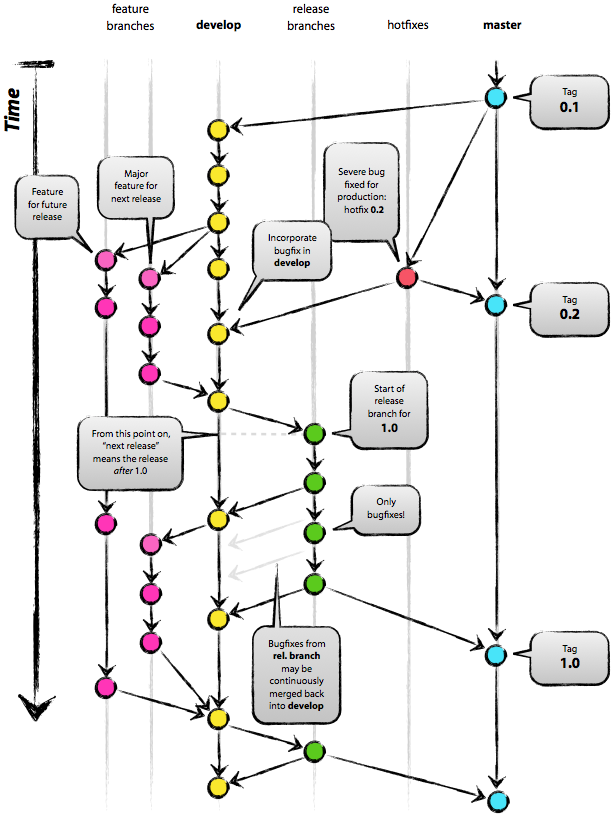
\includegraphics[width=.8\textwidth]{git_branching}
    \column{.55\textwidth}
    \begin{itemize}
    \item Strive for ``useful nonlinearity.''
    \item Develop separate feature sets on separate branches; merge them back to master when complete.
    \item Minimize or eliminate periodic or unnecessary \texttt{merge} commits.
    \item \texttt{rebase} feature branches on top of master before
        merge + push
    \item Rebasing public branches is bad\texttrademark.  Complete the
        shared branch, branch from the shared branch locally,
        \texttt{rebase} from target, then \texttt{merge}
    \end{itemize}
  \end{columns}
    \small
    \begin{itemize}
    \item \url{http://nvie.com/posts/a-successful-git-branching-model}
    \end{itemize}
\end{frame}


%===============================================================================
\section{Development and Testing}
%===============================================================================


\begin{frame}{Issue, Pull Request Tracking}
  \begin{center}
    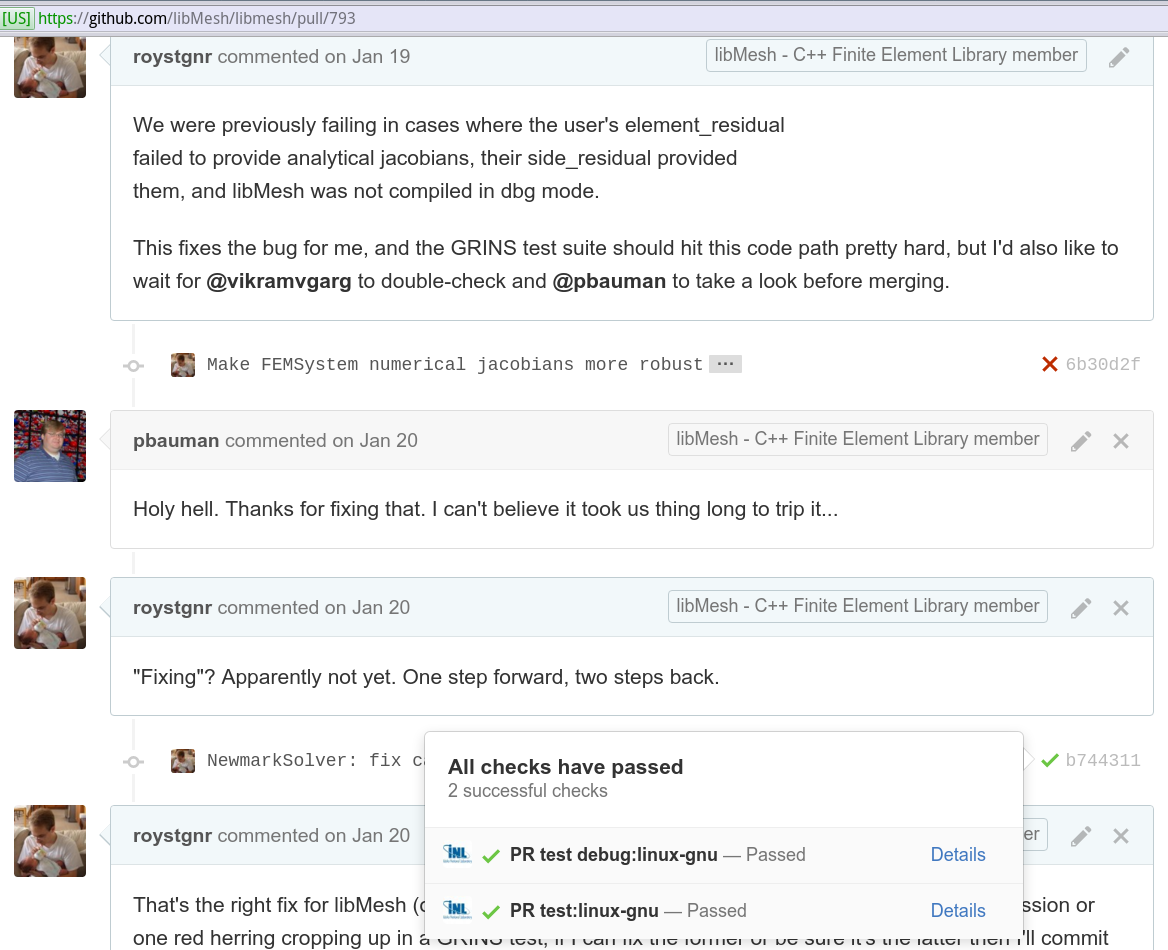
\includegraphics[width=.8\textwidth]{github_ticket}
  \end{center}
\end{frame}


\begin{frame}[fragile]
\frametitle{Tracking API Changes}

\begin{block}{API versions easily proliferate...}
%\begin{minted}[fontsize=\footnotesize]{c++}
\small
\begin{semiverbatim}
#if PETSC_VERSION_LESS_THAN(3,1,0)
  ierr = MatGetSubMatrix(matrix->mat(),
           _restrict_to_is, _restrict_to_is_complement,
           \alert{PETSC_DECIDE}, MAT_INITIAL_MATRIX, &submat1);
#else
  ierr = MatGetSubMatrix(matrix->mat(),
           _restrict_to_is, _restrict_to_is_complement,
           MAT_INITIAL_MATRIX, &submat1);
#endif
\end{semiverbatim}
%\end{minted}
\end{block}

\begin{itemize}
	\item Maintain a wide range of external compatibility
        \begin{itemize}
            \item Dropped PETSc 2.3.3 (2007) support for libMesh 1.0 (2016)
            \item C++11 shims
        \end{itemize}
	\item Limit \libMesh{} API changes
\end{itemize}

\end{frame}

\begin{frame}
\frametitle{Signaling API Changes}
\begin{block}{Development practices}
\begin{itemize}
	\item Old, new APIs {\emph{overlap}}
	\item Easier with C++ function overloading, default arguments
	\begin{itemize}
		\item Adding \texttt{f(a,b)} does not preclude keeping
			\texttt{f(a)}
		\item Adding \texttt{f(a,b=default)} can replace
			\texttt{f(a)}
	\end{itemize}
\end{itemize}
\end{block}

\begin{block}{Runtime warnings}
\begin{itemize}
	\item {\texttt{libmesh\_experimental()}} \quad (in-flux APIs)
	\item {\texttt{libmesh\_deprecated()}} \quad ($\sim$1 year, 1-2 releases)
\end{itemize}
\end{block}

\begin{block}{Examples}
\begin{itemize}
	\item {\texttt{OStringStream} workaround class}
	\item {\texttt{Parallel::} global functions}
\end{itemize}
\end{block}


\end{frame}



\begin{frame}[t]{Regression Testing}
  % Slide notes:
  % * MOOSE (and dependent apps) have regression test suites which must all pass before a commit
  %   is allowed to merge into MOOSE-stable
  % * Shown on the right is a summary of the regression tests for MOOSE itself.
  % * The tests are all designed to be relatively "fast" (and can be run in parallel) so the CI system doesn't get bogged down.
  \begin{columns}
    \column{.2\textwidth}
    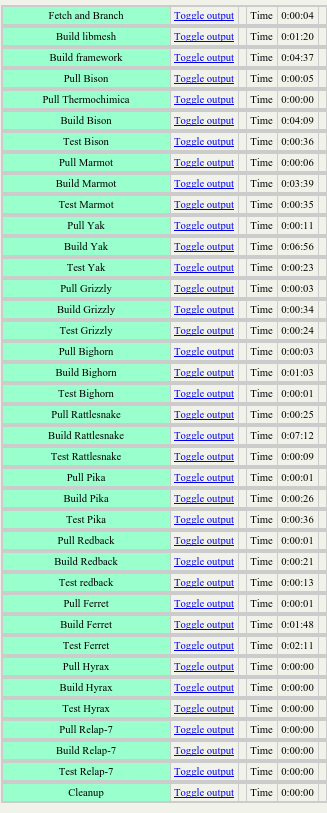
\includegraphics[width=\textwidth]{moose_tests}

    \column{.75\textwidth}
    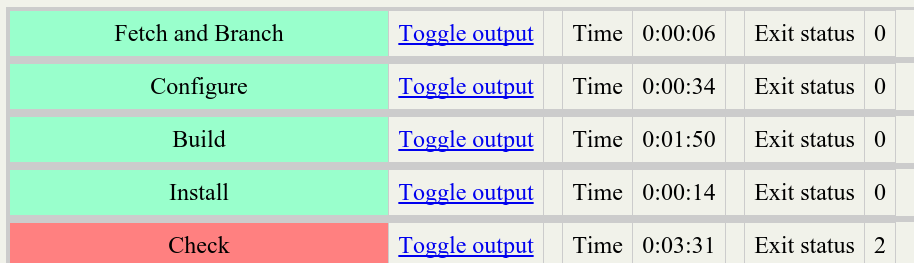
\includegraphics[width=\textwidth]{civet}
    \begin{itemize}
    \item $\sim 7000$ internal assertions in debug mode
    \item $\sim 60$ core example applications 
    \item $\sim 400$ unit tests
    \item Configurations: optional features, index width, ParallelMesh,
                          solver package, scalar precision, -np, --n\_threads
    \item Middleware, application test suites
    \end{itemize}
  \end{columns}
\end{frame}


\begin{frame}[fragile]
\frametitle{Assertions}
{\footnotesize
\begin{verbatim}
libmesh_assert(c < _variables.size());
libmesh_assert(s < elem->n_sides());
libmesh_assert((ig >= Ug.first_local_index()) &&
               (ig < Ug.last_local_index()));
libmesh_assert(requested_ids[p].size() == ghost_objects_from_proc[p]);

libmesh_assert(obj_procid != DofObject::invalid_processor_id);
libmesh_assert(mesh.is_prepared());
MeshTools::libmesh_assert_valid_node_procids(mesh);

libmesh_assert(neigh->has_children());
libmesh_assert(error_estimator.error_norm.type(var) == H1_SEMINORM ||
               error_estimator.error_norm.type(var) == W1_INF_SEMINORM)
libmesh_assert(number_h_refinements > 0 || number_p_refinements > 0);
\end{verbatim}
}

\pause

\begin{itemize}[<+->]
\item Trust preconditions/postconditions, not any of your users
\item Earlier errors are easier errors
\item Exceptions!  Stack traces!  Line numbers!
\end{itemize}

\end{frame}



\begin{frame}{Manufactured Solution Testing}

  (Finding unknown unknowns)

  \begin{columns}[c]
    \begin{column}{6cm}

      \begin{block}{Verification of FIN-S hypersonics code}
        \small
        \begin{itemize}
        \item \small FANS, Spalart-Allmaras
          
        \item Derivative:
          \begin{equation}
            \nonumber  
            \frac{d(sa)}{dx} = \frac{1}{\rho}*\left(\frac{d(\rho *sa)}{dx} - sa \frac{d\rho}{dx}\right)
          \end{equation}
          
        \item In code:
          \begin{equation}
            \nonumber  
            \frac{d(sa)}{dx} = \frac{1}{\rho}*\frac{d(\rho *sa)}{dx} - sa \frac{d \rho}{dx}
          \end{equation}
          
        \end{itemize}
      \end{block}
    \end{column}

    \begin{column}{5cm}
      \begin{center}
        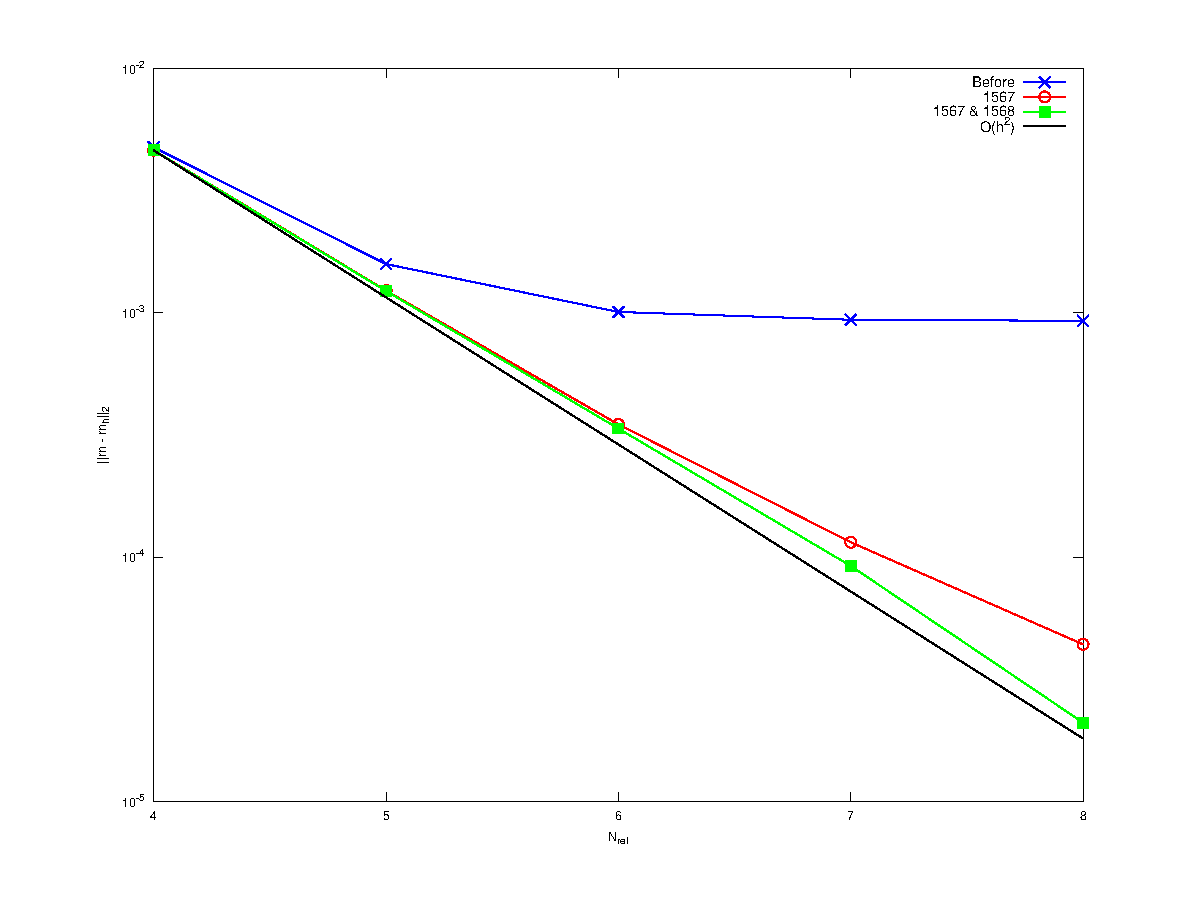
\includegraphics[scale=.3]{sa_bug} \\
      \end{center}
    \end{column}

    \end{columns}

    \vspace{5mm}

    Manufactured Analytical Solution Abstraction library:

    \url{https://manufactured-solutions.github.io/MASA/}

\end{frame}


%===============================================================================
\section{Build Systems}
%===============================================================================


\begin{frame}{Autotools, Pros and Cons}
  % Slide notes:
  % * We've been using autoconf forever
  % * Automake, libtool are much more recent, more controversial
  % * We looked at scons, cmake
  % * We keep bootstrap output in git so RCS users don't need automake
  % * But now build system changes are much more annoying
\begin{columns}
\column{.5\textwidth}
\begin{block}{Autoconf}
	\begin{itemize}
		\item \pro{Manages feature selection}
			\begin{itemize}
				\item 50+ {\texttt{--enable-foo}} options
			\end{itemize}
		\item \pro{Portability tests, workarounds}
		\item \con{POSIX shell dependence}
	\end{itemize}
\end{block}

\begin{block}{Libtool}
	\begin{itemize}
		\item \pro{DLL management in install}
		\item \pro{Broader shared library support}
		\item \pro{Easily used via automake}
		\item \con{Trickier in-build debugging}
	\end{itemize}
\end{block}

\column{.4\textwidth}
\begin{block}{Automake}
	\begin{itemize}
		\item \pro{dist, check, install targets}
		\item \pro{Out-of-source builds}
		\item \pro{\emph{Standardized conventions}}
		\item \con{More difficult METHODS support}
		\item \con{``bootstrap'' process}
		\begin{itemize}
			\item \con{Do users have autotools?}
			\item \con{Custom scripts for libMesh}
		\end{itemize}
	\end{itemize}
\end{block}

\end{columns}

\end{frame}


%===============================================================================
\begin{frame}
\frametitle{Acknowledgements}

Recent contributors:
\begin{columns}

\column{.45\textwidth}

\begin{itemize}
\item David Andrs
\item Paul Bauman
\item Vikram Garg
\item Derek Gaston
\item Dmitry Karpeev 
\end{itemize}

\column{.45\textwidth}
\begin{itemize}
\item Benjamin Kirk
\item David Knezevic
\item Cody Permann
\item John Peterson 
\item Sylvain Vallaghe
\end{itemize}

\end{columns}

\vspace{5mm}

Useful resources:
\begin{itemize}
\item libMesh: \url{https://libmesh.github.io/}
\item GRINS: \url{https://grinsfem.github.io/}
\item MOOSE: \url{https://mooseframework.org/}
\item MASA: \url{https://manufactured-solutions.github.io/MASA/}
\end{itemize}

\begin{columns}[c] 
\begin{column}{.5\textwidth} 
\begin{block}{}
\center{Questions?}
\end{block}
\end{column}
\end{columns}


\end{frame}

 
\end{document}

% LocalWords:  SVN df bibtex benkirk eigen bd API contrib mpi fef rpc
% LocalWords:  cfd ebaa webpage aa petsc xdr LibMeshInit constness bc
% LocalWords:  dphi eac adjoint bugfixes UnsteadySolver aac simpson
% LocalWords:  Wshadow Nonlinearity Epetra vtkDoubleArray bac fe fae
% LocalWords:  ce VTK cato da netcdf SCC GitHub nonlinearity rebase
% LocalWords:  Rebasing hg svn ci Trac versa
